\section{Akvizicija zvuka}
\label{sec:acq}

Podsustav za akviziciju zvuka je usko vezan uz platformu na kojoj
je sustav implementiran zbog toga što je zadužen za komunikaciju 
sa sustavom koji prikuplja stvarne signale sa senzora (mikrofona).
ESP32 Lyrat Development Board \cite{lyrat}, na kojem je sustav
implementiran, na sebi ima već ugrađen mikrofon i audio kodek
s kojim je moguće komunicirati putem I2S protokola. Na slici
\ref{pic:esp} prikazan je blok dijagram ESP32 razvojne platforme.

\begin{figure}[htb]
    \centering
    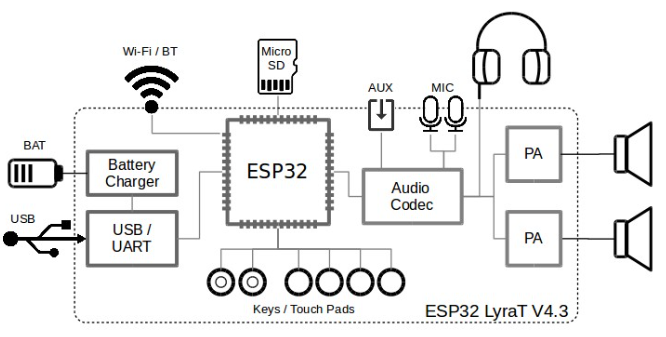
\includegraphics[width=0.75\linewidth]{Chapters/struktura_sustava/akvizicija/lyrat.png} 
    \caption{ESP32 Lyrat \cite{lyrat}}
    \label{pic:esp}
\end{figure}

Najvažniji dio razvojne platforme je upravo ESP32-WROVER-E mikrokontroler
na kojem je cjelopukni sustav za prepoznavanje govornih naredbi 
implementiran. Upravo on je zadužen za komunikaciju s ES8388 
audio kodekom \cite{es8388}. ES8388 je integrirani sklop koji na spomenutoj
platformi služi za analogno-digitalnu (engl. ADC) te digitalno-analognu 
(engl. DAC) pretvorbu, tj. upravljanje audio ulazom (mikrofon) te audio
izlazom (AUX konektor). Mikrokontroler putem I2C sučelja konfigurira kodek,
dok konkretne zvučne signale uzima putem I2S sučelja. Budući da je ESP32 Lyrat
platforma prilagođena razvoju audio sustava, konfiguracija i puštanje u pogon
akvizicije zvuka je vrlo jednostavno. U programskom kodu \ref{code:ES8388init}
prikazana je inicijalizacija kodeka.\\

\begin{lstlisting}[language=C++, caption=Inicijalizacija kodeka]
    audio_board_handle_t board_handle = audio_board_init();
    audio_hal_ctrl_codec(board_handle->audio_hal, AUDIO_HAL_CODEC_MODE_ENCODE, AUDIO_HAL_CTRL_START);
\end{lstlisting}
\label{code:ES8388init}

Sav posao koji se nalazi iza prikazanih naredbi, obavlja ESP-ADF
(Espressif Audio Development Framework). To je biblioteka koja pojednostavljuje
razvoj aplikacija vezanih za obradu zvuka kao što je akvizicija, kodiranje i 
dekodiranje različitih formata audio zapisa te komunikacija s računalom ili 
memorijskom karticom.
Nakon inicijalizacije kodeka i definiranja konfiguracije postavki I2S komunikacije,
potrebno je samo pokrenuti protočni akvizicijski sustav (engl. pipeline), 
a to je prikazano u programskom kodu \ref{code:pipeline}.\\

\begin{lstlisting}[language=C++, caption=Pokretanje akvizicijskog sustava]
    ESP_LOGI(TAG, "Creating i2s stream");
    audio_element_handle_t i2s_stream_reader;
    i2s_stream_cfg_t i2s_cfg = I2S_STREAM_CFG_DEFAULT();
    i2s_cfg.type = AUDIO_STREAM_READER;
    i2s_cfg.i2s_port = I2S_NUM_0;
    i2s_cfg.i2s_config = i2s;
    i2s_stream_reader = i2s_stream_init(&i2s_cfg);

    ESP_LOGI(TAG, "Creating audio pipeline");
    audio_pipeline_handle_t pipeline;
    audio_pipeline_cfg_t pipeline_cfg = DEFAULT_AUDIO_PIPELINE_CONFIG();
    pipeline = audio_pipeline_init(&pipeline_cfg);
    audio_pipeline_register(pipeline, i2s_stream_reader, "i2s");
    audio_pipeline_run(pipeline);
\end{lstlisting}
\label{code:pipeline}

Frekvencija otipkavanja postavljena u konfiguraciji iznosi 16000 Hz što
je dovoljno za ovakav tip sustava \cite{wardentinyml}.
Nakon pokretanja akvizicijskog podsustava, sve što je preostalo je uzimati nove
podatke s kraja protočne strukture podsustava. Konstantno uzimanje novih podataka, tj. komunikacija
s ES8388 kodekom, odvojeno je u posebnu dretvu. Na taj način programski je 
odvojena akvizicija sirovih podataka (sirovi u smislu da nisu još obrađeni ni
na kakav način) od ostatka sustava. Ovaj podsustav je proizvođač novih podataka,
dok je ostatak sustava potrošač (također jednodretven). Sve što je preostalo je
ubaciti pouzdan i efikasan način komunikacije između. Za tu svrhu odabran je
kružni međuspremnik (engl. ring buffer). On omogućuje asinkrono pisanje u njega
te čitanje iz njega. Implementacija takve strukture dostupna je unutar FreeRTOS-a 
\ref{ringbuff}. 


\begin{lstlisting}[language=C++, caption=Razred AudioRecorder]
class AudioRecorder
{
    private:
        uint32_t sampleRate;
        RingbufHandle_t ringBuffer;
        TaskHandle_t captureAudioHandle;
        static void captureAudioTask(void* pvParameters);
    public:
        AudioRecorder(uint32_t sampleRate) : sampleRate(sampleRate), 
                                             ringBuffer(NULL), 
                                             captureAudioHandle(NULL) {}
        uint32_t getSamples(int16_t* samples, size_t numOfSamples);
};
\end{lstlisting}
\label{code:AudioRecorder}

Opisani podsustav za akviziciju u programskom kodu zapakiran je u razred imena 
AudioRecorder \ref{code:AudioRecorder}. Prema van, razred nudi metodu potpisa
\texttt{uint32\_t getSamples(int16\_t* samples, size\_t numOfSamples)} koja 
omogućuje dohvaćanje proizvoljnog broja \texttt{uint16\_t} podataka jer 
se akvizirani zvučni signal sprema upravo u tom obliku. Zbog ovakve strukture
ovog podsustava, sve što je potrebno u glavnoj petlji sustava je stvaranje objekta
razreda AudioRecorder, alociranje spremnika za dohvaćanje podataka te kontinuirano
pozivanje opisane funkcije koja kao argumente prima pokazivač na alocirani spremnik
te željeni broj audio uzoraka.

Spomenuta modularnost ostvarena je tako što je cijela funkcionalnost akviziranja
novih zvučnih uzoraka sadržana u opisanom razredu. Pokretanje cjelokupnog sustava
na drugoj platformi koja ima drugi audio kodek, drugačiji mikrofon ili se samo 
radi o drugom mikrokontroleru bit će moguće pisanjem novog razreda koji
prati zadano sučelje.